\section{Implementation} \label{sec:implementation} 

\subsection{Data collection}\label{sec:implementation:collection}
% - to be aligned with Gleb
% - see in the drive

% Paragraph 1
% - why do we use imagenet1k? (1 paragraph)
% - why is imagenet1k better than other datasets? (same paragraph) 
% 
We select the ImageNet-1k dataset, a widely recognized benchmark dataset in computer vision that is particularly well-suited for training and evaluating deep learning models for image classification~\cite{paperswithcode_imagenet, DBLP:journals/cacm/KrizhevskySH17}. We selected ImageNet-1k due to its large-scale diversity, high-quality annotations, and extensive use in prior research. Compared to smaller datasets like CIFAR-10 or MNIST, ImageNet-1k offers greater variety in object classes and real-world complexity, making it a better choice for training robust and generalizable models.

% Paragraph 2
% - present google landmark issue and how imagenet was better (1 paragraph)
% probably not necessary on second thought, we have enough words already.

% Paragraph 3
% - how did we collect and process this data? (1 paragraph)
%
We accessed and loaded the ImageNet-1k from the HuggingFace \texttt{datasets} library \cite{jain2022hugging}, which provides convenient access to a wide variety of public datasets. However, ImageNet-1k is massive, containing over 1.2 million high-resolution images, and loading the entire dataset into RAM is infeasible on most hardware, especially on non-supercomputers \ref{nfr5}. Thus, we implemented a custom class that lazily loads images from disk only when images are needed for a training batch, thus keeping memory usage manageable and scalable across systems. This class also ensures compatibility with PyTorch. Besides, we use PyTorch’s \texttt{DataLoader} to create batched data streams for efficient training and evaluation, with appropriate shuffling and parallel loading via multiple workers to maximize throughput during training.

\subsection{Data pre-processing}\label{sec:implementation:augmentation}
% Paragraph 1 - 50 words
% Explain why do we need pre-processing in the first place and what if we were to not have it + references
% link with the FRs / NFRs (especially accuracy) 2,4,5
%
Pre-processing is essential in deep learning pipelines to standardize input data, improve model generalization, and reduce computational complexity. Without pre-processing, raw images may contain variations in lighting, scale, and background noise, leading to inconsistencies and lower classification accuracy \cite{DBLP:journals/pieee/LeCunBBH98}. Furthermore, pre-processing ensures that models learn meaningful representations rather than overfitting to irrelevant pixel-level details. Standardization also enables efficient training by improving convergence rates and reducing training instability \cite{DBLP:journals/cacm/KrizhevskySH17}. All these pre-processing techniques, corroborated with the other training techniques, contribute to meeting the accuracy requirements \ref{nfr2}.

% Paragraph 2 - 75 words
% Which pre-processing/augmentation methods did we use, explain what they do, and why we chose these methods specifically
%
Each image is resized to $224 \times 224$ pixels and normalized using the standard ImageNet mean and standard deviation values. Resizing ensures compatibility with widely used architectures such as ResNet and EfficientNet, which expect this input size. Normalization ensures that pixel values are distributed consistently across all input samples, improving stability during gradient updates. These transformations prevent scale variations from affecting the model’s predictions while maintaining the original dataset's inherent diversity.

% Paragraph 3 - 75 words (p2 continued)
% If we didn't augment the data - why not?
% perhaps: imagenet-1k is already so big it's not necessary
% or perhaps: our model is 4 different efficientnets whose outputs are averaged, so does this leave us vulnerable to overfitting? and data augmentation might make it easier to overfit?
% or perhaps: recreating a compute-limited environment?
%
Data augmentation techniques such as random cropping, flipping, or rotation were deliberately omitted. ImageNet-1k is already a large-scale dataset with extensive intra-class variability, reducing the risk of overfitting. Additionally, our experimental setup involves comparing SiMo, a simple-model approach, against CoMo integrating multiple architectures \ref{nfr3}. To ensure a fair comparison, we kept the training conditions consistent between both models. Furthermore, our resource constraints \ref{nfr5} necessitate an efficient training process, and omitting augmentation speeds up training while still allowing generalization due to ImageNet’s inherent diversity.

\subsection{Data division}\label{sec:implementation:division}

% Paragraph 1 - 50 words
% Describe some background, why we need a split, how is this done in large-scale projects, etc.
% how should this be done --
Proper data division is crucial for training robust machine learning models \cite{Goodfellow-et-al-2016}. In large-scale projects, datasets are typically split into training, validation, and test sets to ensure that models generalize well beyond the training data. A well-structured split prevents data leakage and overfitting while enabling fair performance evaluation. The division process should mimic real-world scenarios, ensuring that the validation and test sets contain diverse samples representative of unseen data.

% Paragraph 2 -  100 words
% What specific data split proportion we used, and why.
We followed the official ImageNet-1k dataset split, which provides predefined training, validation, and test sets. This ensures consistency with prior benchmarks and prevents unintentional biases that could arise from manually re-splitting the data. The majority of the data (1,181,167 images) is allocated to the training set, allowing the model to learn diverse patterns. The validation set (50,000 images) is used for hyperparameter tuning, while the test set (100,000 images) remains untouched until final evaluation, ensuring an unbiased measure of model performance. Using this established split also allows for direct comparison with existing research, while still complying with best practices in the community.

% Paragraph 3
% What data split we did NOT use and why. + compare why our approach is better
We did not employ alternative splitting strategies, such as an arbitrary 80/10/10 or k-fold cross-validation. The ImageNet-1k dataset is already balanced and large enough, thus making additional re-splitting redundant, even detrimental to models' performance. K-fold cross-validation \cite{luntz1969estimation}, while beneficial for smaller datasets, would significantly increase computational costs \ref{nfr5} without offering a meaningful advantage. By adhering to the standard ImageNet-1K split, we ensure that our results align with broader research findings and maintain comparability while optimizing training efficiency.

% \begin{figure}
%     \centering
%     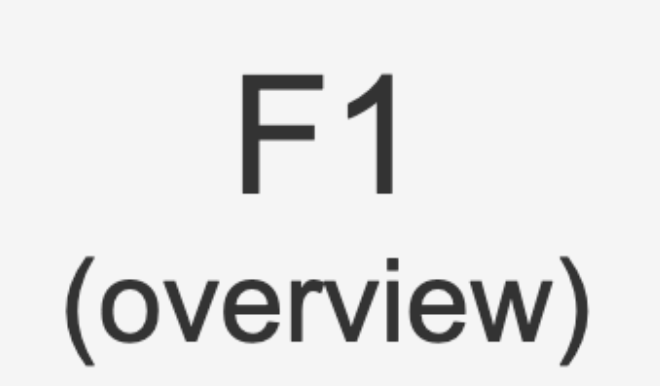
\includegraphics[width=0.95\linewidth]{figures/f1.png}
%     \caption{Example of data augmentation or whatever.}
%     \label{fig:augmentation}
% \end{figure}
% \lipsum[1]


\subsection{Model implementation and training}\label{sec:implementation:training}
% Write about L2 regularization (weight decay), adam optimizer, on what machine it was trained, epochs, hyperparameters, etc.

Both SiMo and CoMo follow the same training approach to ensure consistency among experiments and that the only difference between the models is their architecture.

The training loop consists of forward propagation, loss computation using the cross-entropy loss function, backpropagation, and weight updates. The models were trained for 200 epochs with a maximum batch size that fit on the GPU (we conducted several test runs for hyperparameter choice that showed that it was the most optimal configuration), where each epoch consisted of iterating over 256 dataset batches. The validation phase followed each training epoch, during which the models were evaluated on a separate validation dataset to monitor their generalization performance. To optimize model performance, we occasionally updated the hyperparameters through a trial-and-error approach based on validation performance \ref{fr3}.

To optimize the model’s learning process, we employed the Adam optimizer \cite{kingma2014adam}, which adapts the learning rate for each parameter, enhancing training efficiency and convergence. Additionally, we used a cosine annealing learning rate scheduler to adjust the learning rate dynamically throughout training. This scheduler reduces the learning rate gradually, preventing abrupt changes that could lead to instability and allowing smooth convergence.

While regularization strategies such as L1, L2 regularization, or dropout can be helpful to avoid overfitting, our test runs have shown that, for our use case, these techniques only slow down the training, without offering a clear performance advantage. Due to our large dataset size, even the most complex studied model does not show signs of overfitting for the selected training time.

We chose to train each EfficientNet from scratch because the training resources are an essential metric for our research. After individually training each component, we combined individual sub-components into the final CoMo ensemble. Due to computational constraints, we were unable to train the EfficientNet models for an extended time-period. Training was halted after 200 epochs; at this point, models showed only minor improvements with increased training time. However, based on existing baselines, we argue that longer training could improve accuracy up to 80\%, or even beyond~\cite{paperswithcode_imagenet}. This limitation means that our final reported results do not fully reflect the potential of the EfficientNet-based models. Still, the findings provide a meaningful comparison between different architectures under limited-resource conditions.

During training, the training data was periodically stored using the Wandb~\cite{wandb} framework. After training, SiMo and CoMo performance was tested using a test set to ensure the models could generalize well to never-before-seen data.